\documentclass{article}
\usepackage[utf8]{inputenc}


\usepackage[margin=1in,top=1in,bottom=1in]{geometry}
\usepackage[pdftex]{graphicx}
\usepackage{tikz}
\usetikzlibrary{shapes,arrows,patterns,decorations.pathreplacing, decorations.markings,positioning,calc,decorations.pathmorphing}
\usepackage{setspace}
\usepackage{epstopdf}
\usepackage{caption}
\usepackage{enumitem}
\usepackage{pdfpages}
\usepackage{placeins}
\usepackage{subcaption}
\usepackage{amsmath}
\usepackage{empheq}
\usepackage{cancel}
\usepackage{xcolor}
\usepackage{etoolbox}
\usepackage{soul}
\usepackage{listings}
\lstset{
       basicstyle=\footnotesize\ttfamily,
       backgroundcolor=\color{lightGray},
       frame=single,
%        basicstyle=\footnotesize\sf,
       captionpos=b,
       tabsize=2,
       keepspaces=true,
       breaklines=true,
       postbreak=\mbox{\textcolor{red}{$\hookrightarrow$}\space},
  }
\usepackage{color}
\definecolor{lightGray}{rgb}{0.95,0.95,0.95}

% The call to include hyperref must be after most of the other packages are called.
% One notable exception it that hyperref must come before cleveref.
% Basically keep these two packages at the end of the \usepackage{} calls, in this order.
\usepackage[pdftex,
            hidelinks,
            pdfauthor={Evan Brunton},
            pdftitle={MAE 3302 --- Project Part 1},
            pdfsubject={Thermodynamics 2}
            ]{hyperref}


\usepackage[capitalize]{cleveref}
\newcommand{\creflastconjunction}{,~and~} % page 12 of the manual to get serial comma correct

\graphicspath{{Figures/}}

\title{Conceptual Design of a Combined Gas Turbine and Steam Turbine Power Plant}

\date{\today}

\author{Evan B, Brunton\\[2ex]
    UCCS Department of Mechanical\\
    and Aerospace Engineering
}

\begin{document}

\maketitle

\pagebreak

\section{Introduction}

    This study will analyze a conceptually combined gas and steam turbine power plant and seek to maximize efficiency. The gas and steam turbine mechanisms will be modeled using ideal Brayton and Rankine thermodynamic cycles with component efficiency factored into the processes. The Brayton cycle models the gas turbine part of the power plant. In the Brayton cycle atmospheric air is first pumped into a combustion chamber raising the pressure of the gas. Combustion is then modeled as heat entering the system in an isobaric process, the temperature rises, but the pressure is constant. The now pressurized and heated gas is put through a turbine to generate work. However, the gas is still extremely hot and more work can be extracted from that energy. The hot gas is then put through a heat exchanger which inputs heat into the Rankine cycle. The Rankine cycle models a steam turbine, which uses the spent heat from the Brayton cycle to heat water into steam that drives a turbine providing more work out. Figure 1 diagrams the inputs/outputs and flow of the two cycles.
    
\begin{figure}[!htbp]
\centering
  \includegraphics[page=1,trim=10mm 40mm 10mm 0mm,clip,width=0.99\textwidth]{Combined Cycle Diagram (1).pdf}
  \caption{}
  \label{fig:epsfig}
\end{figure}

\FloatBarrier

The requested design parameters of the power plant and the efficiency of the components are as follows:

\begin{figure}[htbp]
  \centering
  \begin{subfigure}[t]{0.45\textwidth}
    \centering
  \includegraphics[page=1,trim=0mm 0mm 0mm 0mm,clip,width=0.99\textwidth]{Figures/png2pdf (1).pdf}
  \caption{Component efficencies}
  \label{fig:epsfig}
\end{subfigure}%
  \begin{subfigure}[t]{0.45\textwidth}
  \centering
  \includegraphics[page=1,trim=0mm 0mm 0mm 0mm,clip,width=0.99\textwidth]{Figures/png2pdf.pdf}
  \caption{These are the overall design requirements}
  \label{fig:pdffig}
  \end{subfigure}%
  \caption{}
  \label{fig:testfig}
\end{figure}

\FloatBarrier
In order to increase the efficiency of the entire powerplant both cycles should have their output maximised. The Brayton cycle's efficiency ultimately depends on the pressure ratio. However, as the temperature and pressure increase the costs and feasibility of building a compressor that can handle the high pressure and temperatures rises exponentially the efficiency gain levels off, compressing gas concentrates the heat energy, and compressing at a high temperature takes significantly more energy than a low-temperature gas. Eventually, the work required to compress the atmospheric air overcomes the work generated by the turbine.
A second compressor and inter-cooler can be installed to reduce the work required to compress the gas and the temperature limits of the compressor. Before compressing the gas to its final pressure, the gas is run through a heat exchanger in a constant pressure process. The excess heat can be used in other processes, and not as much work will be required to get the gas to the required pressure.
The Rankine cycle also has to deal with realistic pressure and temperatures requirement determined by our current material science. So increasing temperature and pressure to overcome other losses is not a realistic way to maximize efficiency. The cycle also has to deal with using a two-phase liquid gas mixture throughout the process. A pump can only deal with non-saturated water, and the turbine can only deal with steam at a higher than 90\% quality. So to maximize efficiency one would have to edge their way around the vapor dome, keeping the temperature from getting too high, keeping the compressor from having to over-compress the liquid, and the turbine quality above 90\%.
In order to edge along the vapor dome for the Rankine cycle a reheat cycle and a second turbine can be added. This way temperature doesn't have to get too high and a lower initial temperature can be used. The higher the difference in low and high temperatures will increase the amount of work that can be extracted from the steam. Excess heat energy from other parts of the powerplant, like the combustion chamber, that would have been lost to the atmosphere can be used in this reheat step. This would increase the work generation per unit of energy. This energy comes from burning expensive and polluting gas. 
This report will determine the increase in efficiency from using these extra components. From the results, the efficacy of installing them can be extrapolated from projected fuel savings against the projected cost.

\begin{figure}[!htbp]
\centering
  \includegraphics[page=1,trim=10mm 0mm 10mm 0mm,clip,width=0.99\textwidth]{Figures/Copy of Combined Cycle Diagram.pdf}
  \caption{}
  \label{fig:epsfig}
\end{figure}

\FloatBarrier

\section{ModelingBrayton}

The attached Python script uses CoolProp, a database with experimental values for water and air at incremental states. Using the design requirements of the power plant for all the states of the working fluid/gas can be found. After factoring in the efficiency of the components the enthalpy of the materials can be used to find the work out, work in, and Q-in can be used to find the thermal efficiency of the two cycles. (I will use the real project numbers in submission 3, but for now, they are just random numbers)(kinda feel like reworking the code to use lists instead of lone vars to make it less confusing, and easier to iterate over various pressure ratios and temperatures with the final data to make a big thermal efficiency). The Brayton cycle model with the following initial conditions; a compressor efficiency of 0.95 and a turbine efficiency of 0.93 will have a thermal efficiency of 32.98 \%.
\begin{itemize}
\item  low pressure = 101325 pa
\item Minimum temp of gas = 25 c
\item compressor ratio = 6
\item Maximum temp of gas = 1350 c
\end{itemize}

However, if an intercooler and second compressor are added to the cycle, with the initial compressor having a pressure ratio of 3, and the intercooler cooling the gas to 525c the system will have a thermal efficiency of 35.67 \%.  A 2.69 percent increase may not sound like a lot of savings, but most of the cost of running a power plant is fuel, and a 2.69 \% reduction in fuel costs is a serious amount of money.
\section{ModelingRankine}
The material properties at all states of the Rankine cycle can be found using CoolProp. Then using the enthalpy of the water at the various states work done by the pump, and work out of the turbines can be compared with Q-in.(will update values in submission 3 to project values) Using the following state conditions a pump efficiency of 0.92 and a turbine efficiency of 0.93 the thermal efficiency of the cycle is 37.48 \% is found.
\begin{itemize}
\item  low pressure = 6000 pa
\item high pressure = 10000000 pa
\item low temperature = 30 c
\item high temperature = 440 c
\end{itemize}

However, the minimum quality of the water exiting the turbine is specified to be larger than 90 \%, so as not to break it. Without a reheat and a second turbine, the quality at the turbine exit is 75 \%. If the water leaves the first turbine at 700000 pa and is reheated to the maximum temperature and then sent through a second turbine until it reaches the low pressure the thermal efficiency is 43.20 \%. Not only does the reheating step maintain the quality of the material, so the turbines aren't damaged, but it increases the thermal efficiency by a whole 5.72 \%. Figure 4 shows the modified Temperature and entropy graph of the cycle, the two big drop-offs are the isentropic expansions in the turbines.

\begin{figure}
    \centering
    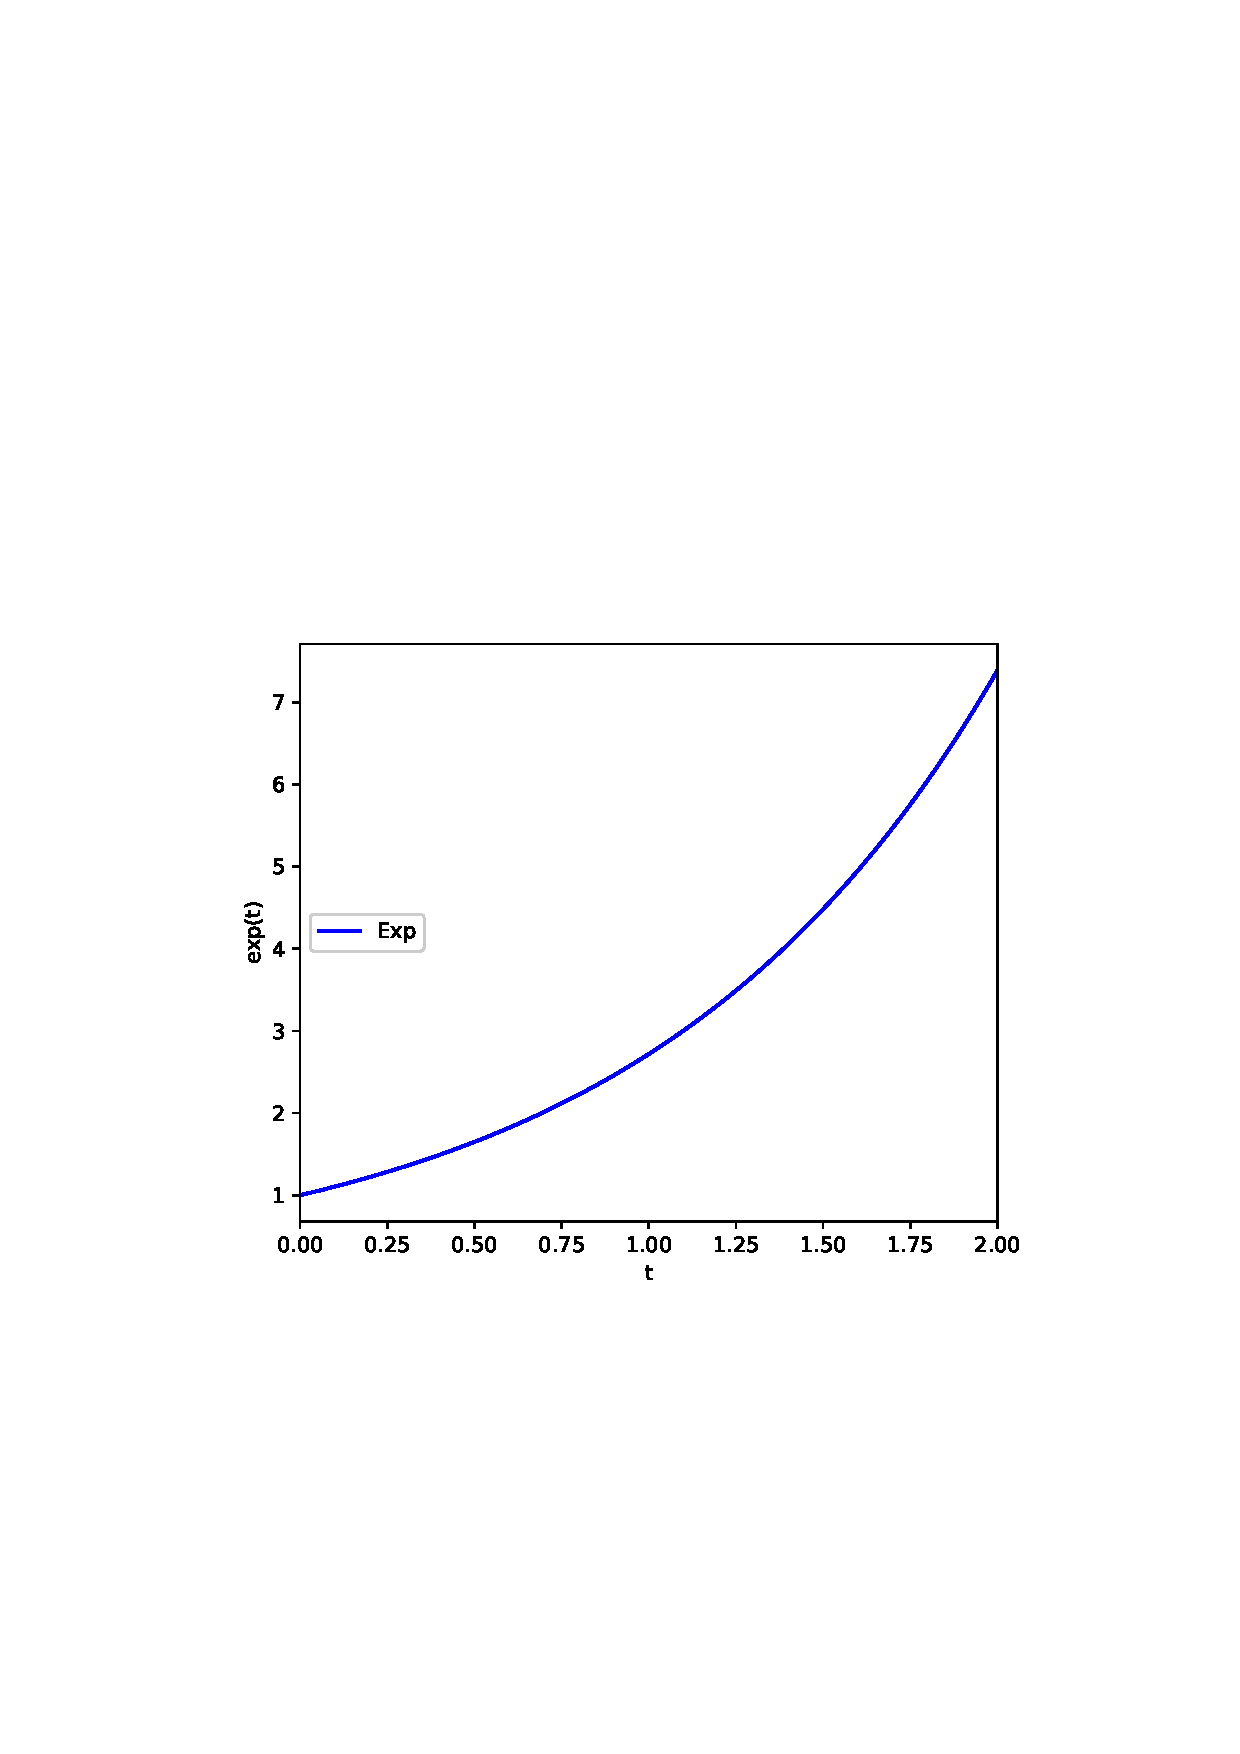
\includegraphics{Fig_test.pdf}
    \caption{Caption}
    
    \label{fig:my_label}
\end{figure}

\FloatBarrier

\section{Modeling Heat Exchanger}
    \[Effectiveness = 0.85\]
   \[Effectiveness = actual Q transfer/ Ideal Q transfer\]
   \[massFlowRateBrayton(h_4 - h_1) = massFlowRateRankine(h_4 - h_1)\]
   \[massFlowRateBrayton(Ideal Q transfer Brayton) = massFlowRateRankine(Ideal Q transfer Rankine)\]
   \[Ideal Q transfer Brayton = Ideal Q transfer\]
   \[actualQtransfer = Effeciveness * massFlowRateRankine(Ideal Q transfer Rankine) / massFlowRateBrayton\]



\section{Results}

This is my results, //will elaborate


Include minimum calculated quality and efficiency of Rankine with and without the reheat cycle. I need to edit the graph to include labels with states.

\section{Conclusions}

This is my conclusion

\appendix

\FloatBarrier % To keep all figures before the references

% produces the bibliography section when processed by BibTeX
\bibliography{Paper_template_bib_file}
\bibliographystyle{aiaa}


\section*{Code Listing}

\lstinputlisting[language=Python]{Great_Code.py}






\end{document}
